\chapter{Methodology} \label{cp:methodology}

\section{Apparatus} \label{sec:apparatus}
A Schlieren Imaging System is set up to view flow through a converging-diverging nozzle in the test section of the supersonic wind tunnel. 

\begin{figure}[htpb]
    \centering
    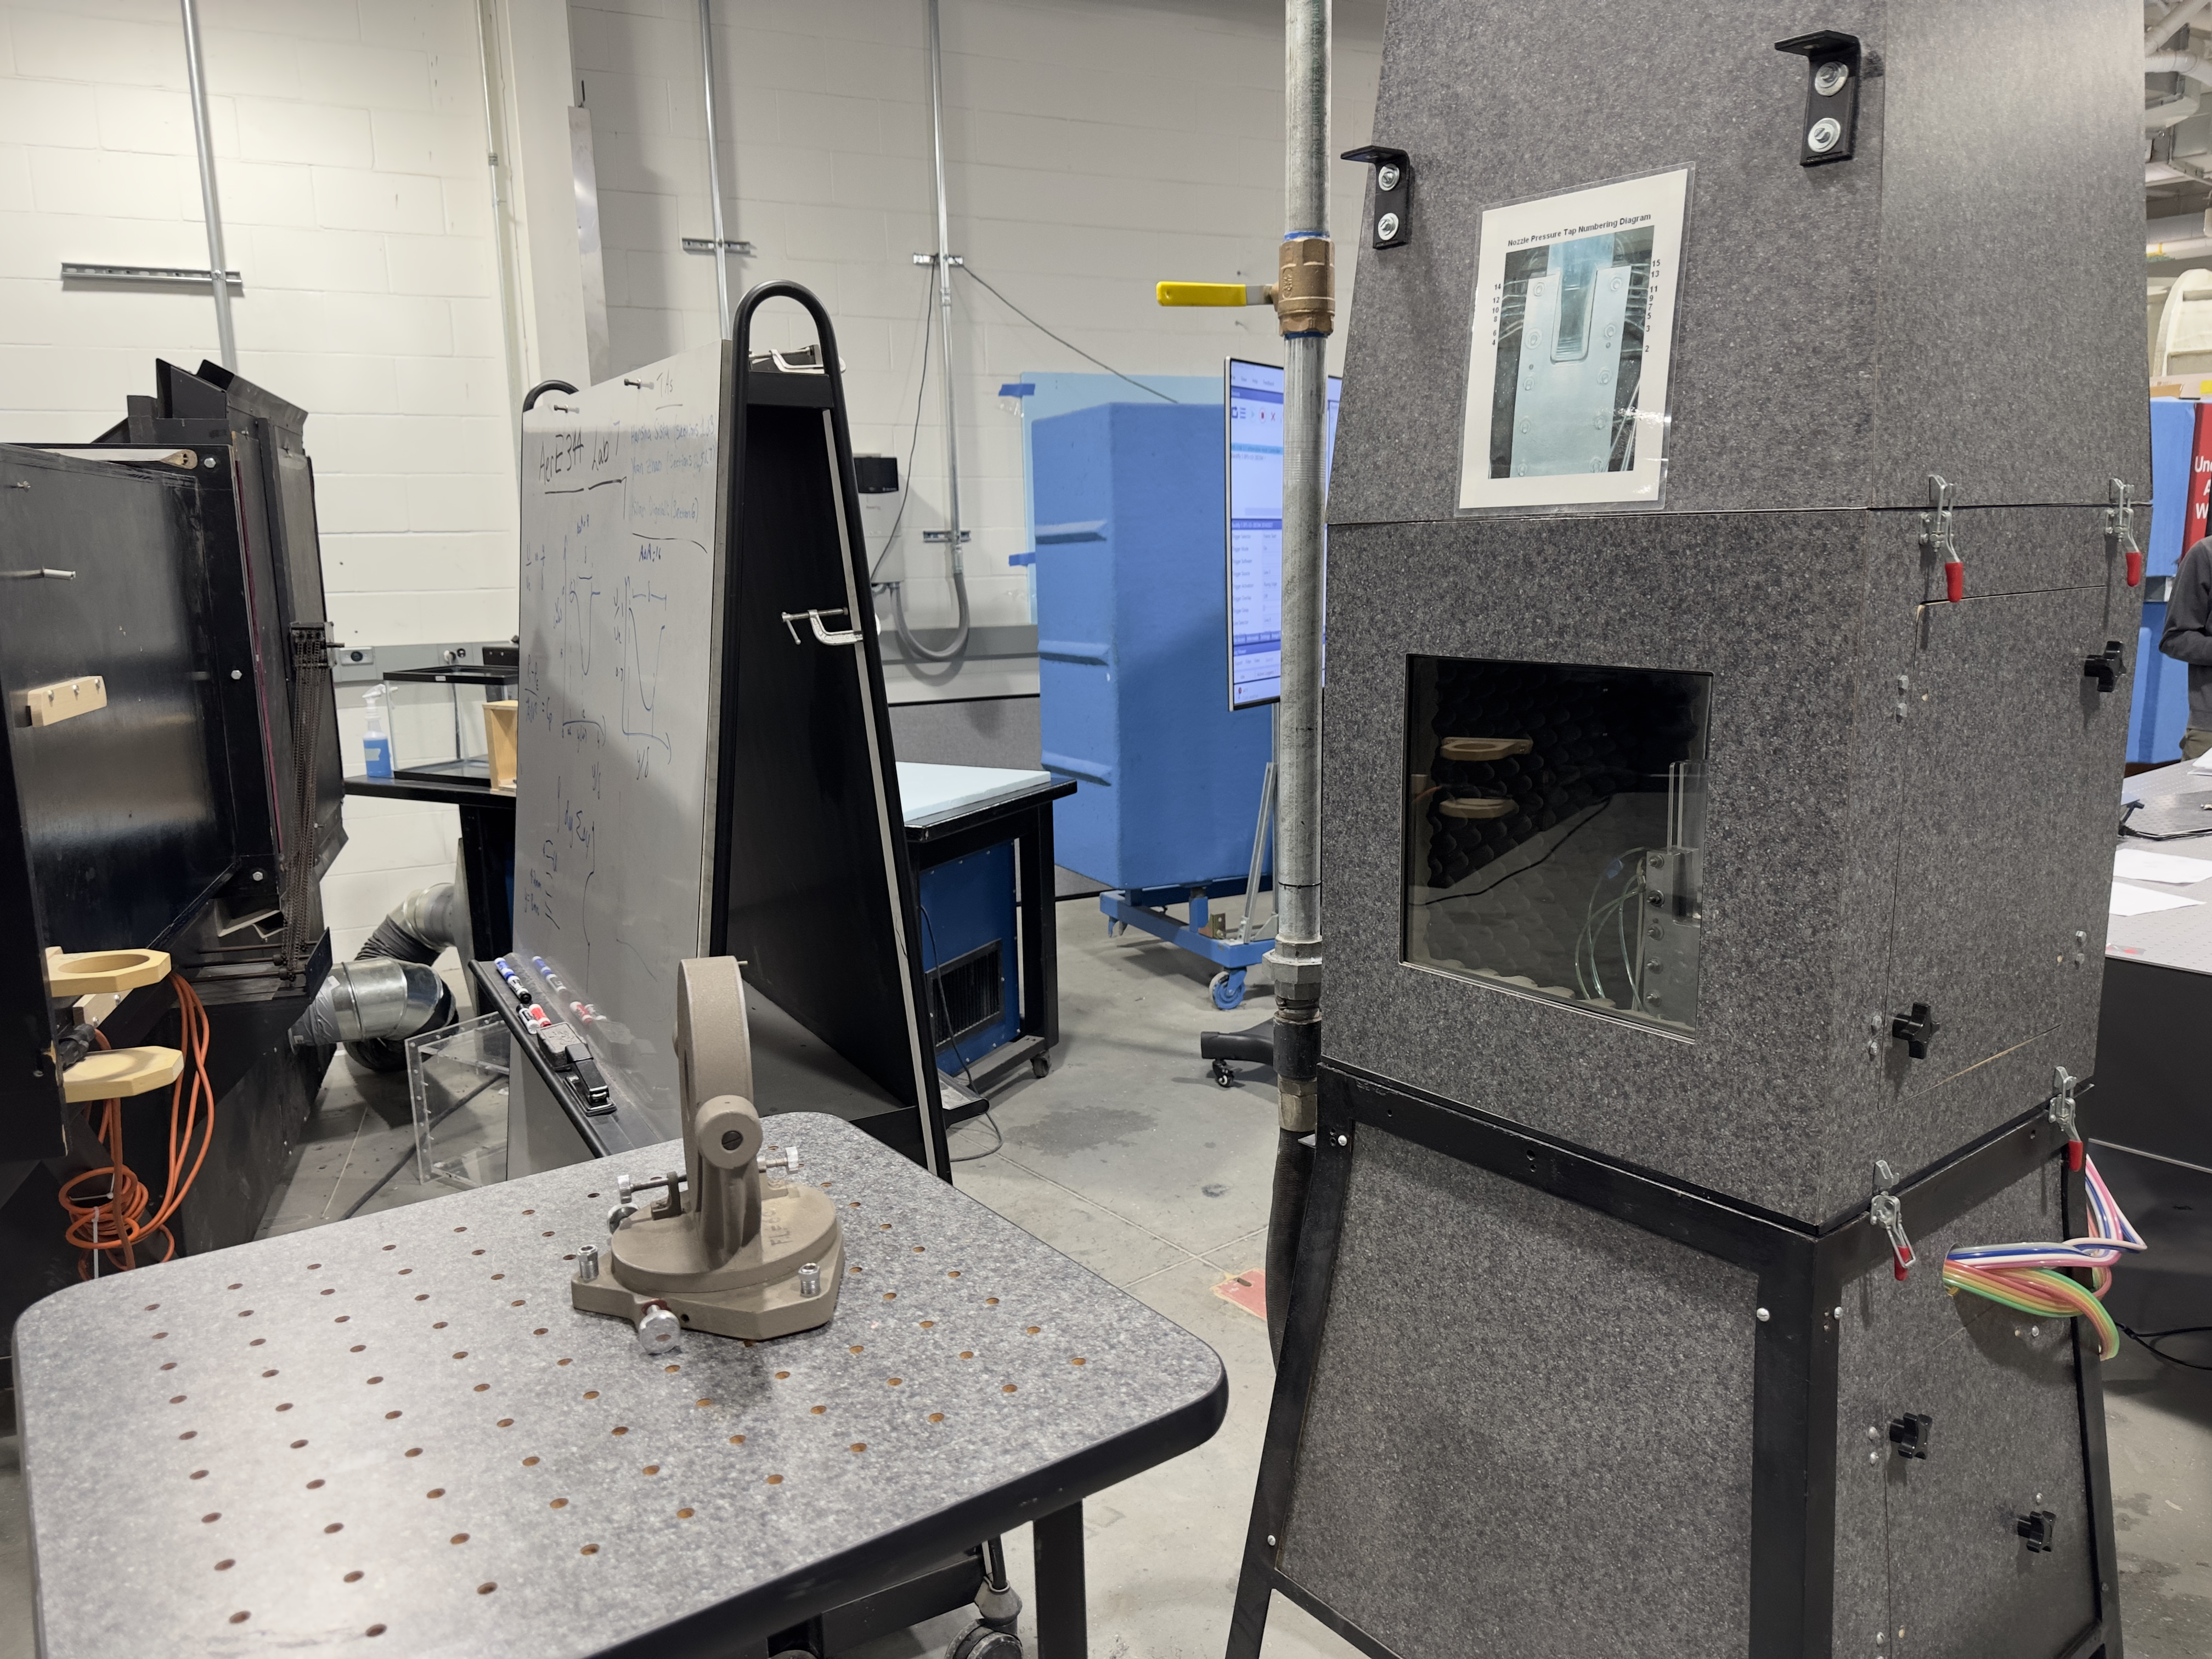
\includegraphics[width=0.75\linewidth]{Figures/back_of_supersonic_wind_tunnel.jpeg}
    \caption{The supersonic wind tunnel.}
    \label{fig:supersonic_wind_tunnel}
\end{figure}

\begin{figure}[htpb]
    \centering
    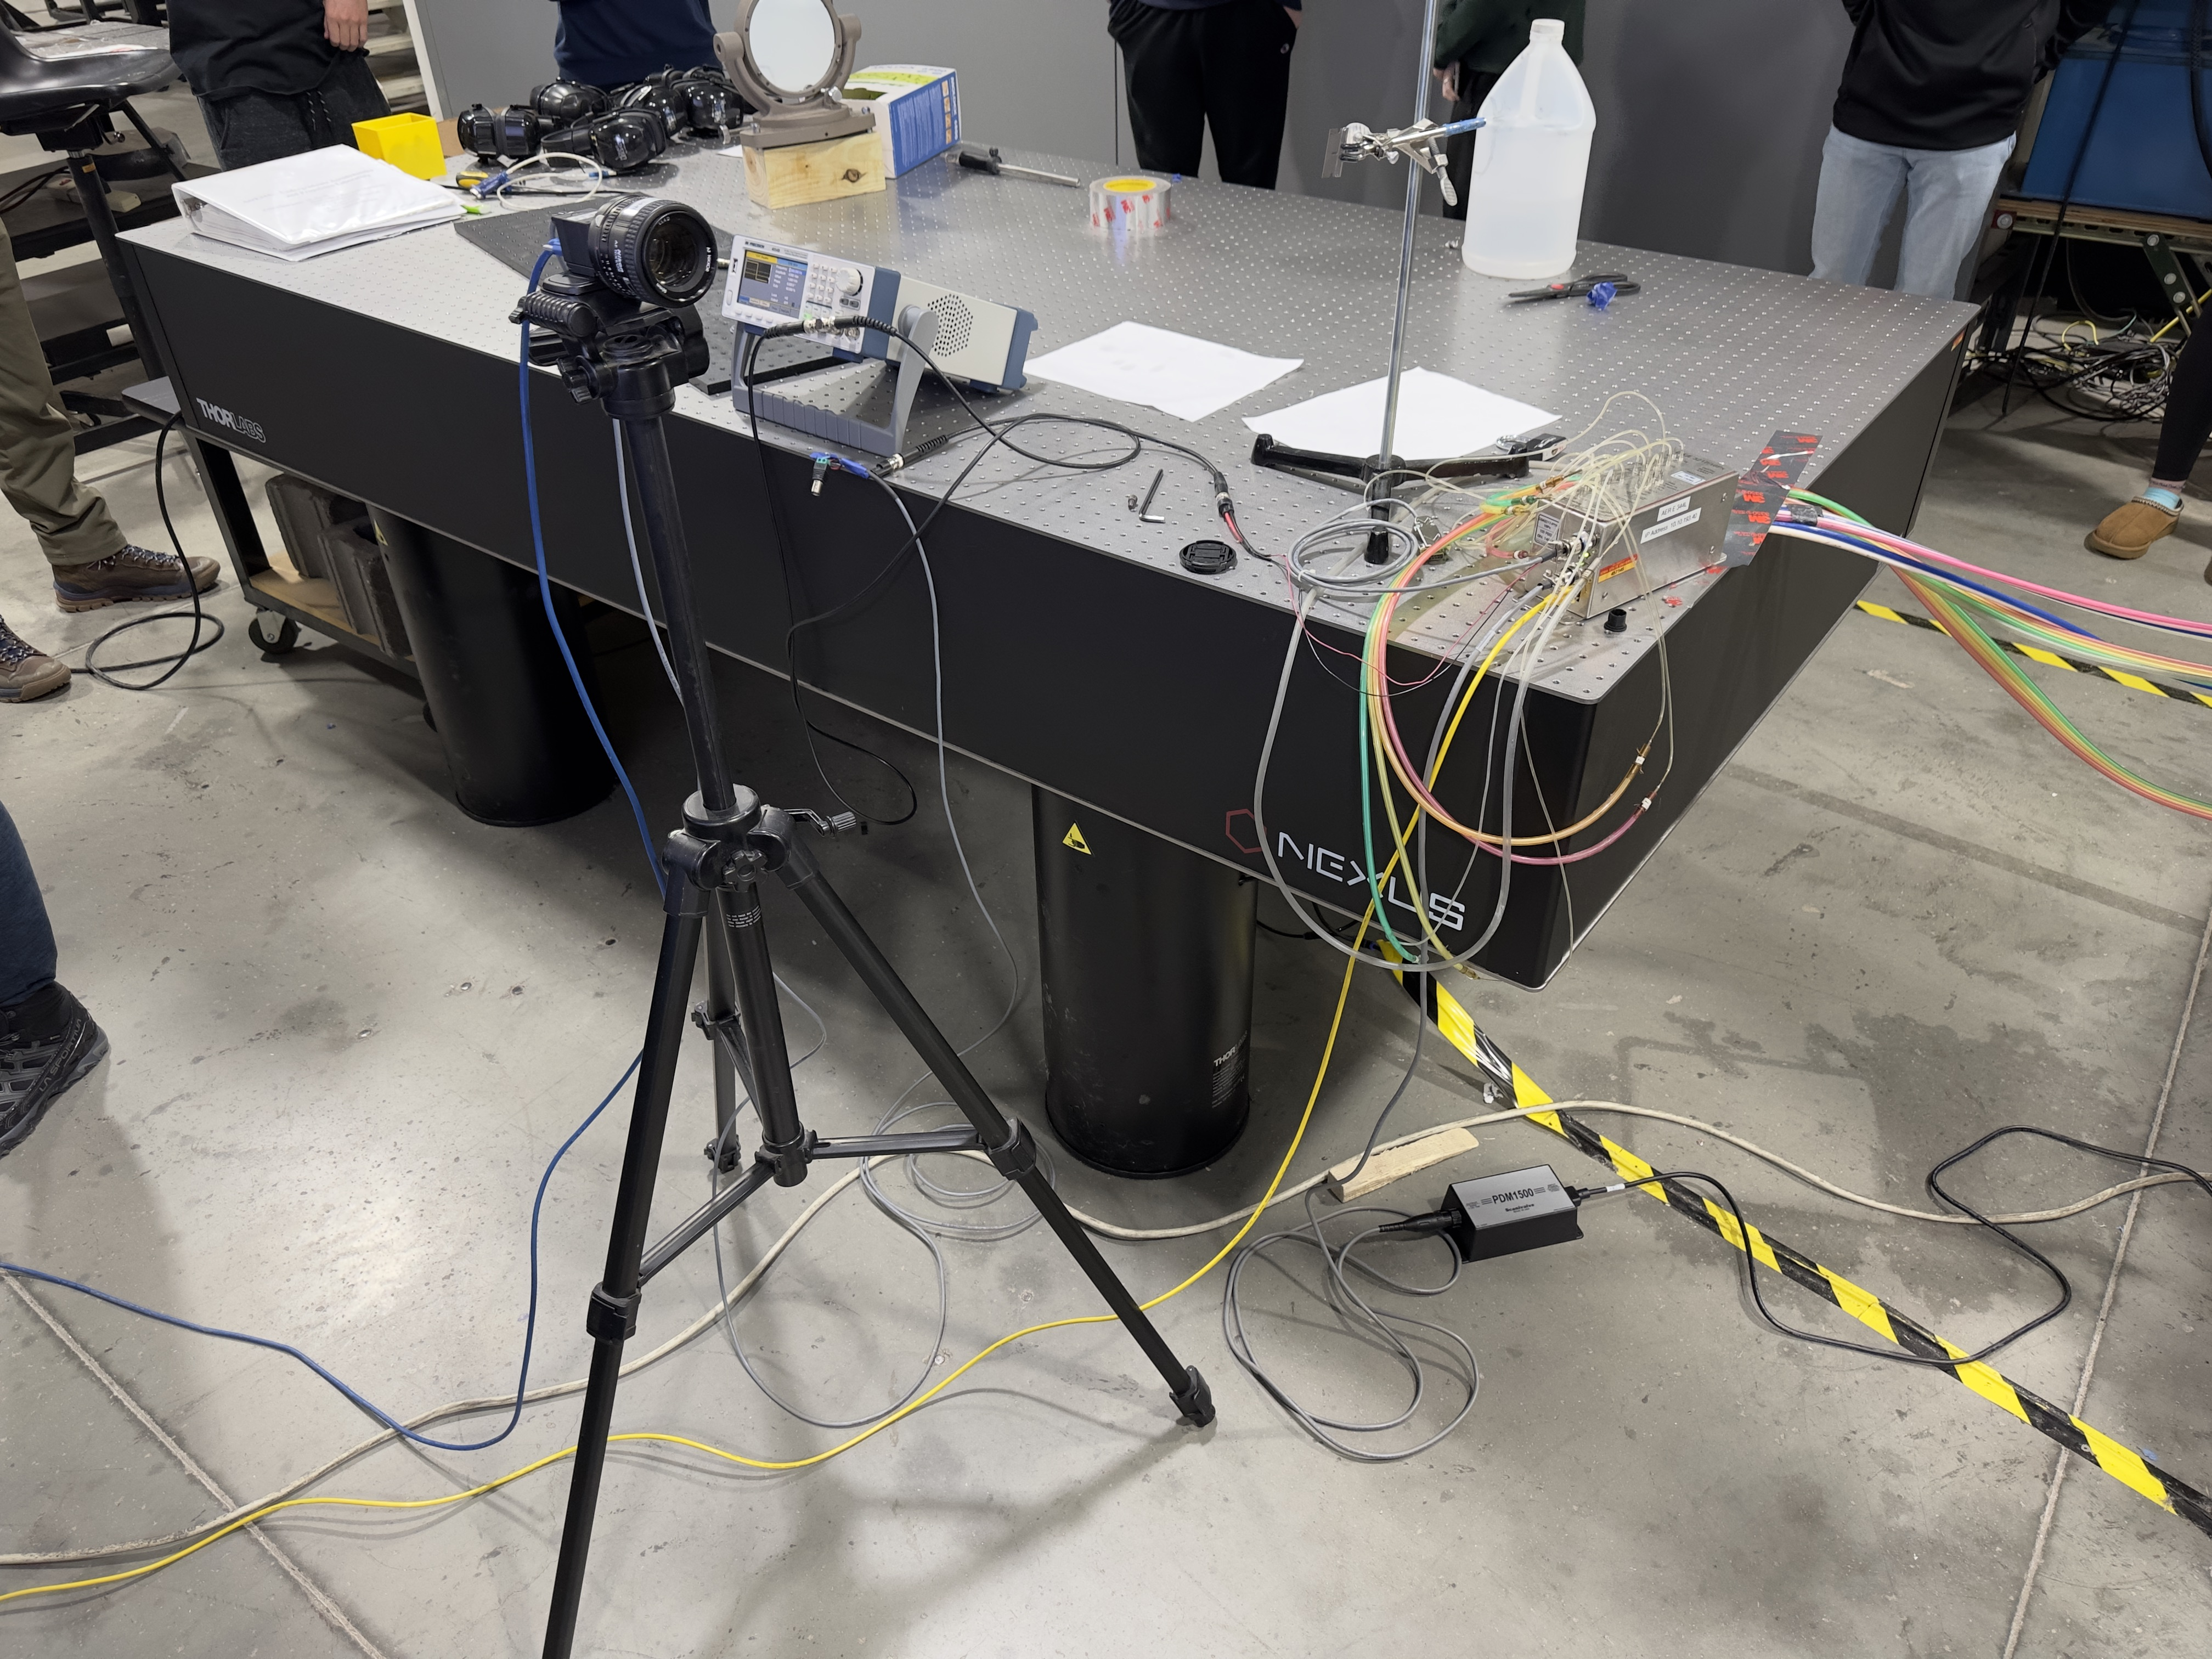
\includegraphics[width=0.75\linewidth]{Figures/camera.jpeg}
    \caption{The camera in the Schlieren configuration takes high-contrast images of the projections of flow passing through the de Laval nozzle.}
    \label{fig:camera}
\end{figure}

\begin{figure}[htpb]
    \centering
    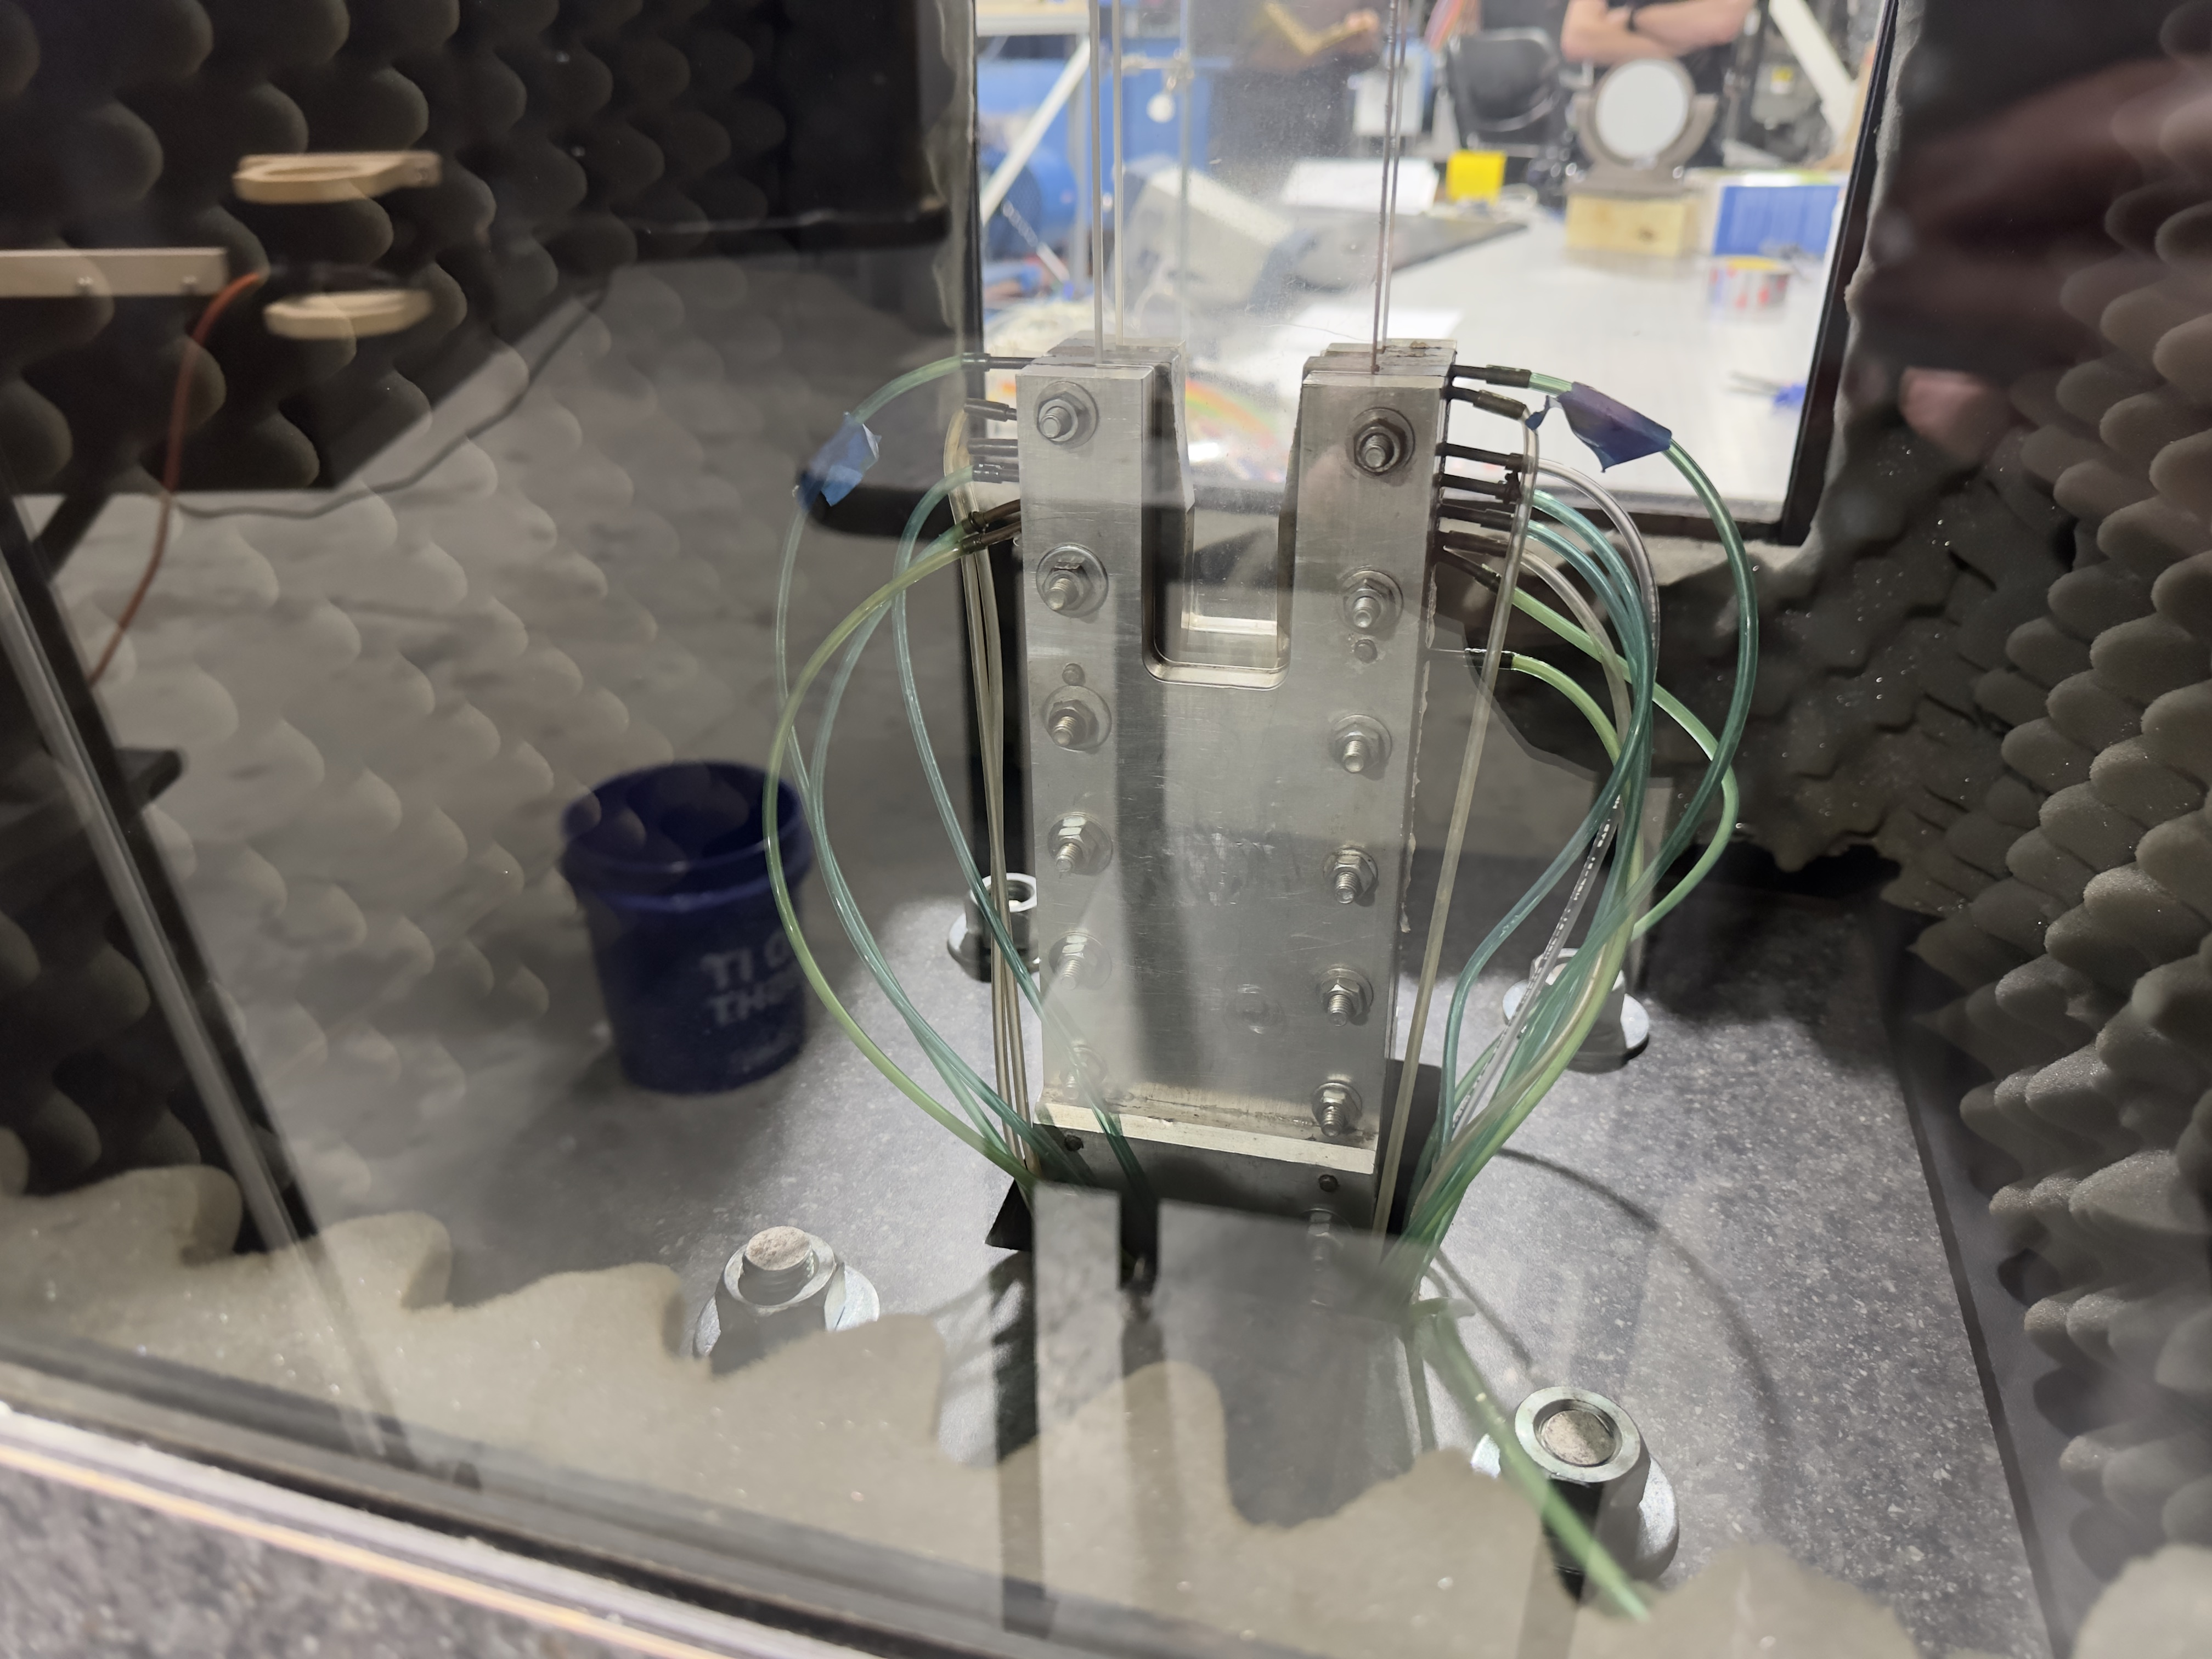
\includegraphics[width=0.75\linewidth]{Figures/de_laval_nozzle.jpeg}
    \caption[The de Laval nozzle in the supersonic wind tunnel.]{The de Laval nozzle in the supersonic wind tunnel. The pressure taps are connected to a pressure transducer which is further connected to the data acquisition computer.}
    \label{fig:de_laval_nozzle}
\end{figure}

\begin{figure}[htpb]
    \centering
    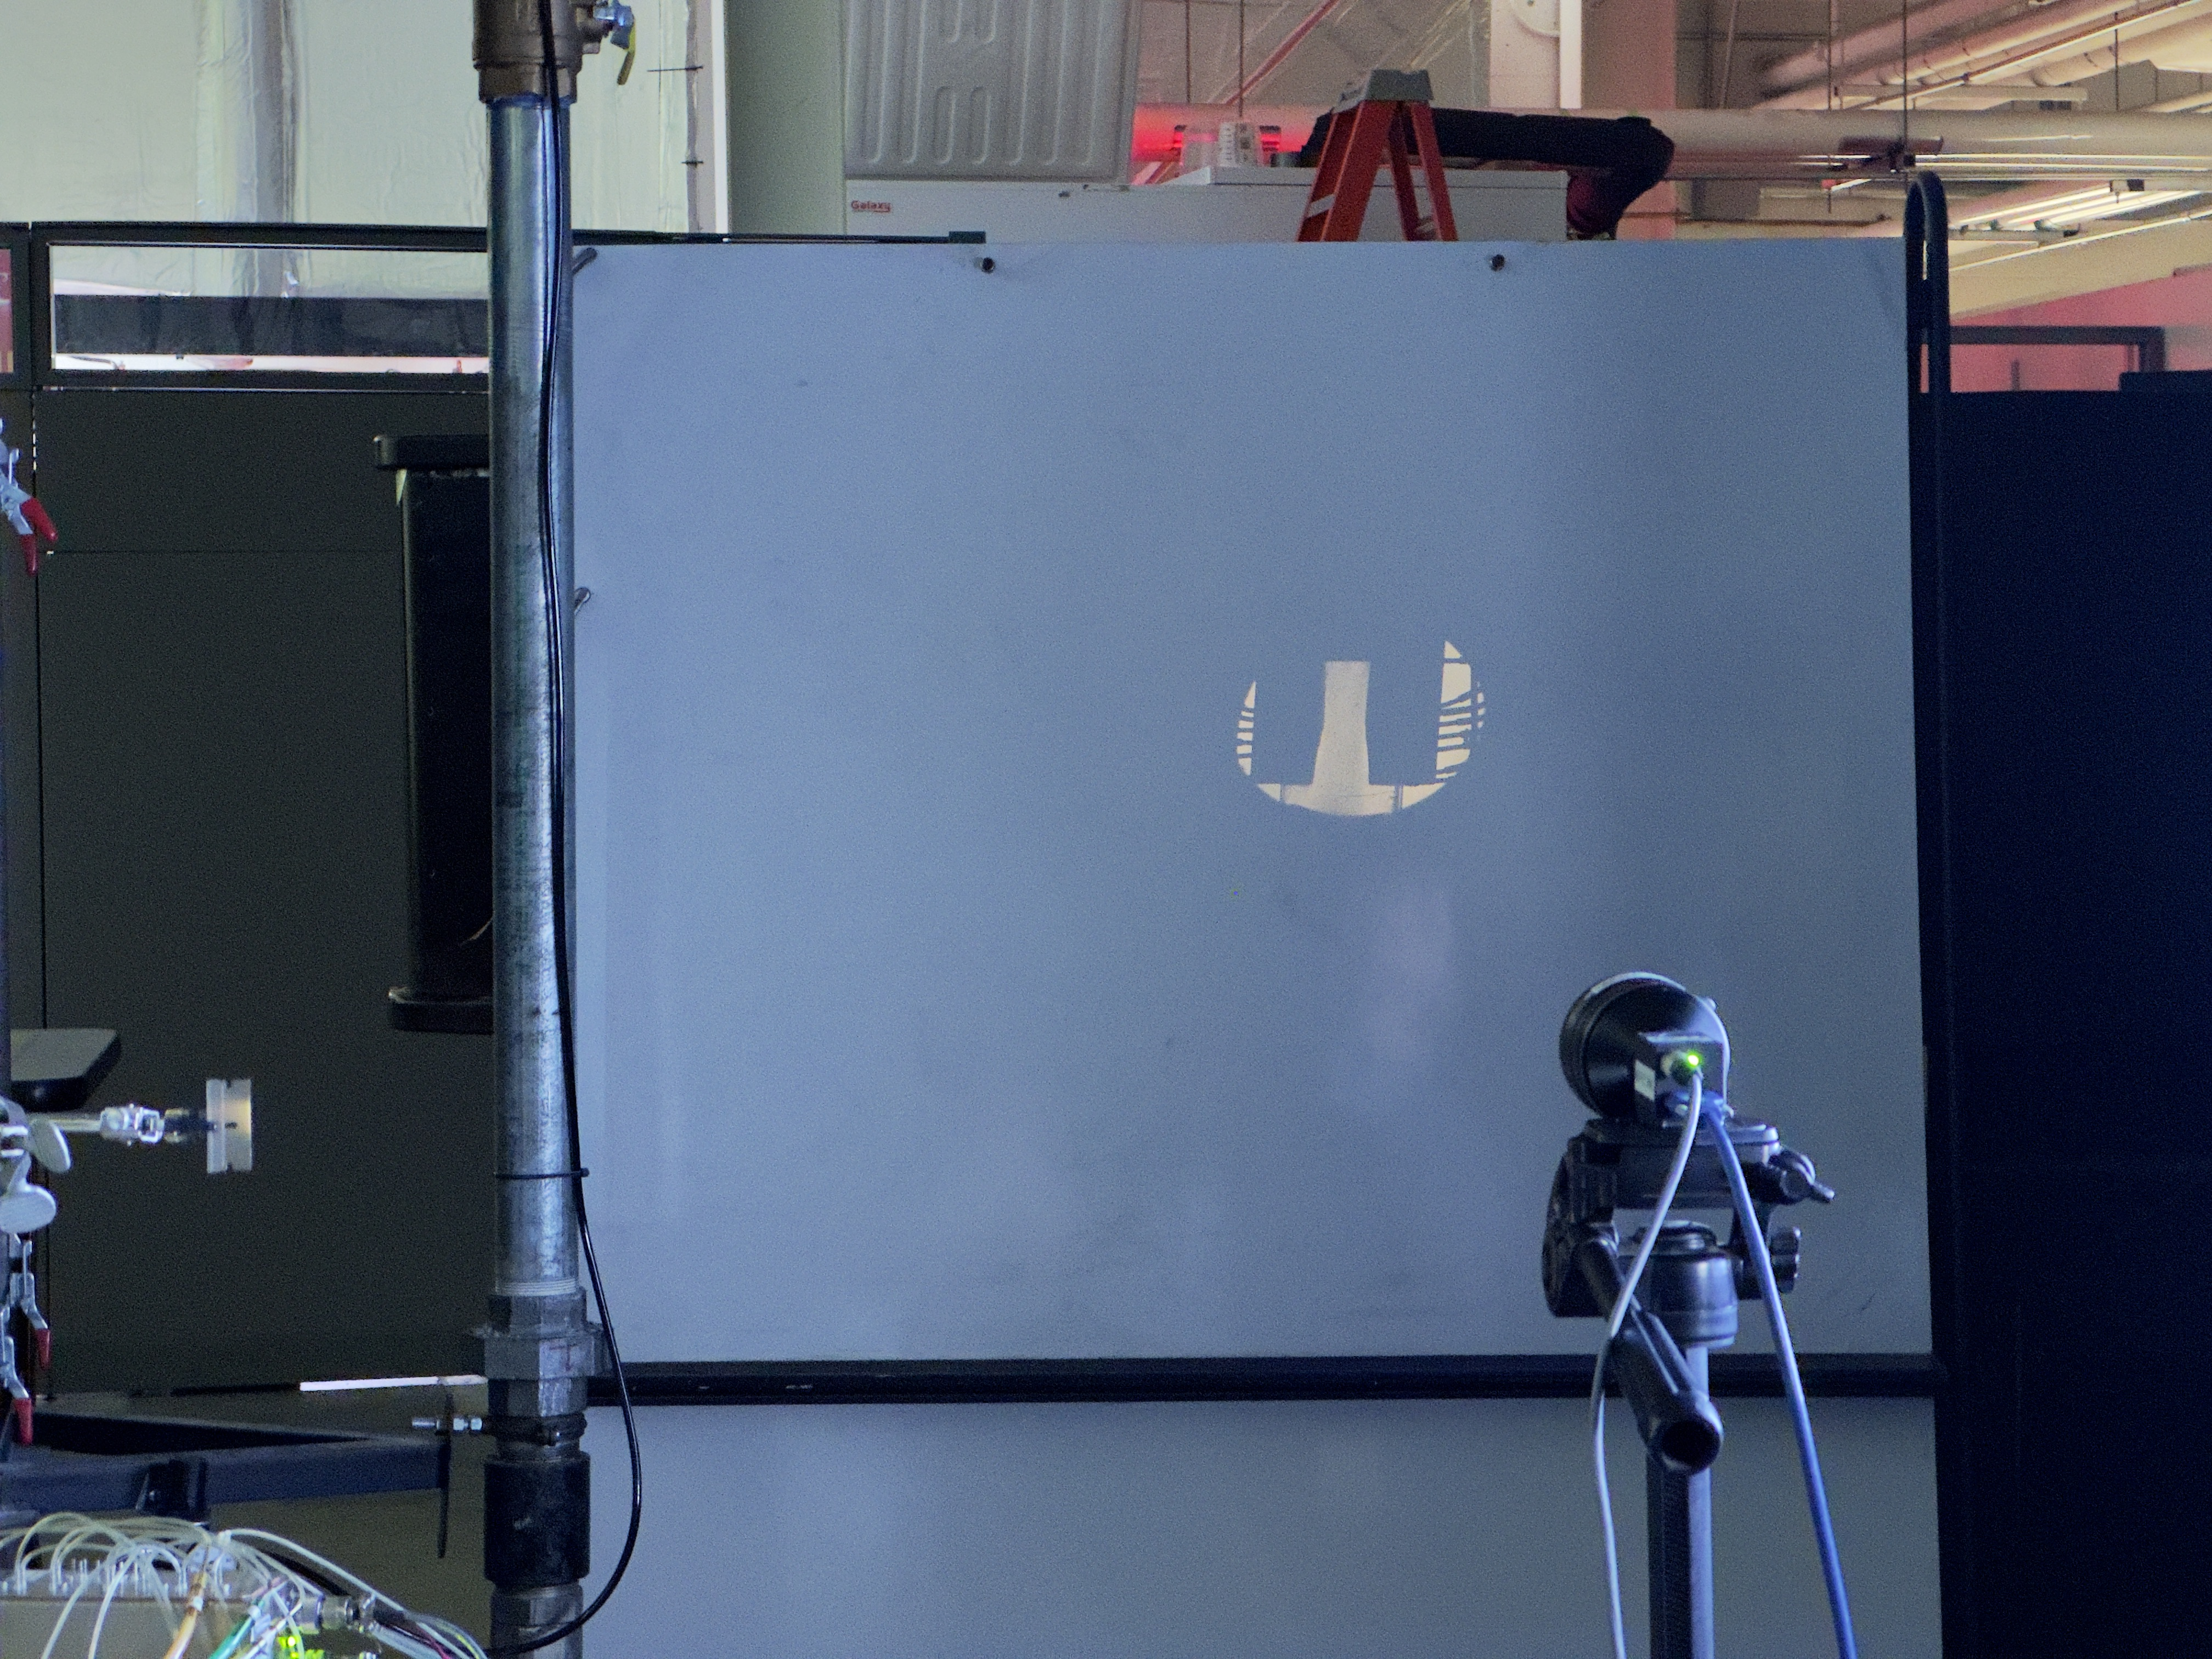
\includegraphics[width=0.75\linewidth]{Figures/schlieren_nozzle.jpeg}
    \caption[A Schlieren projection of the flow moving through the de Laval nozzle being projected onto a white board.]{A Schlieren projection of the flow moving through the de Laval nozzle being projected onto a white board. The camera takes close-up, high-contrast images of the projection.}
    \label{fig:schlieren_projection}
\end{figure}

\section{Procedures} \label{sec:procedures}



\section{Derivations} \label{sec:derivations}

\begin{figure}[htpb]
    \centering
    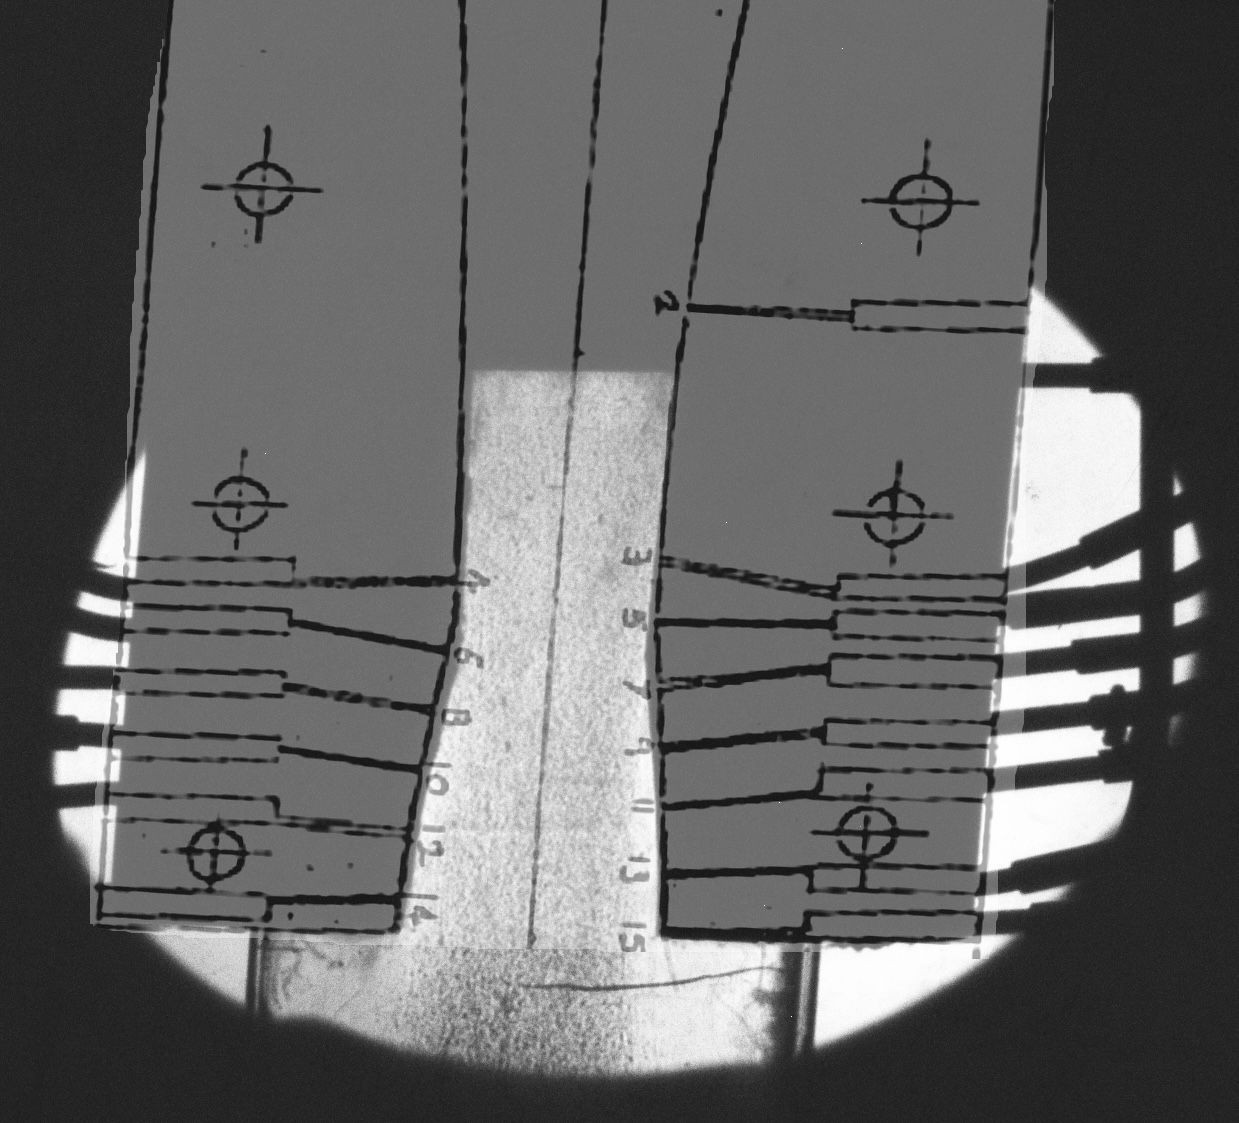
\includegraphics[width=0.75\linewidth]{Figures/Nozzle Overlay with Shock.jpg}
    \caption[An overlay of the de Laval nozzle schematic and an image of the nozzle when a normal shock is present.]{An overlay of the de Laval nozzle schematic and a Schlieren image capture of the de Laval nozzle when the shock is inside the divergent section of the nozzle.}
    \label{fig:schlieren_overlay}
\end{figure}